% storyboard 1 bladzijde
\chapter{Storyboard}\label{chapter:storyboard}

Het volledige storyboard is te zien op figuur \ref{fig:storyboard}. Het storyboard bestaat uit drie fases:

\begin{enumerate}
	\item In de eerste stap heeft de gebruiker de keuze de resultaten te bekijken of om een nieuwe data in te geven.
	\item De optie 'start' brengt de gebruiker naar het eerste invoerscherm. De gebruiker kan nu het aantal uren ingeven dat hij/zij heeft gepresteerd en een rating geven betreffende de kwaliteit van deze prestatie.
	\item Via de optie 'next' komt gebruiker in het laatste scherm terecht. Hier geeft de gebruiker een kwantificatie van zijn gemoedstoestand in op een schaal van $1$ tot $10$.
\end{enumerate}

% http://en.wikibooks.org/wiki/LaTeX/Importing_Graphics
\begin{figure}
  \begin{center}
  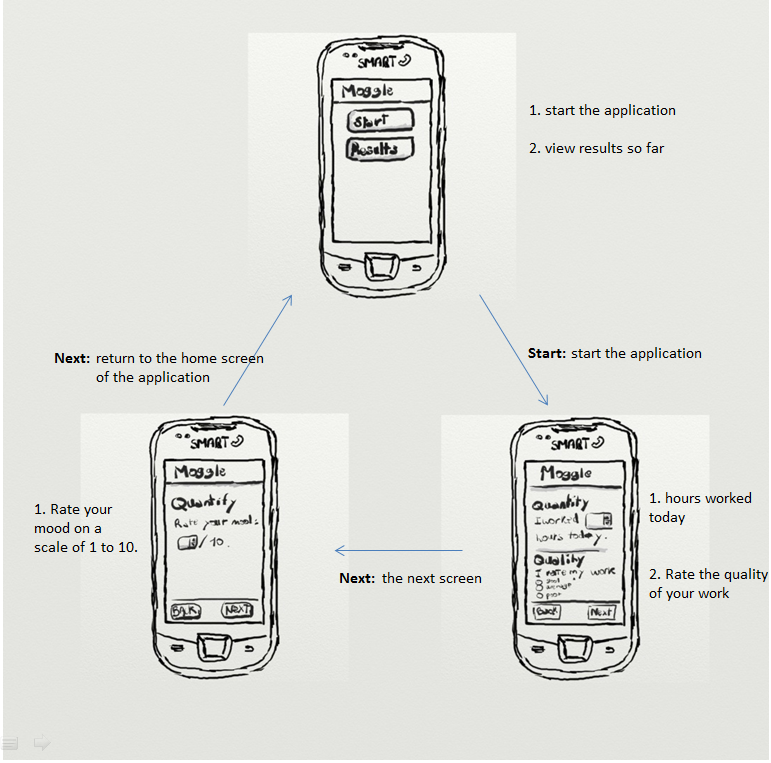
\includegraphics[scale=0.6]{data/storyboard-final}
	\end{center}
  \caption{Moggle storyboard}
	\label{fig:storyboard}
\end{figure}
